\chapter{P7：把受约束 Agent 做成电脑网页工作台}

\section{承上启下}

P6 已经能从自然语言请求得到经过检查的结构化结果，但 CLI 要求使用者理解命令和内部状态。P7 要解决的是“运营人员能不能在电脑浏览器里完成任务”，而不是简单给程序套一个聊天框。

\section{业务问题、输入与边界}

输入是 P6 的流程、商品解析、三类工具、Verifier、引用校验和公开结果合同。目标用户是产品或类目运营。工作台不是消费者选购助手，也不是开放互联网 SaaS，目前只提供 loopback-only 的本地试用边界。

\begin{boundarybox}
开发者自动化、synthetic 合成任务和受控 local 回归，只能证明工程路径。P7 仍为 \statusprogress，因为目标运营用户的\textbf{结构化试用}尚未完成。不能声称已经节省真实工时、改善决策或产生商业收益。
\end{boundarybox}

\section{开发过程}

\subsection{1. 先决定网页可以看到什么}

网页使用独立的 typed public DTO。DTO 可以先理解成“给浏览器看的安全表格”，不直接暴露内部 \texttt{AgentState}、商品映射、真实引用、密钥或路径。字段和值都经过闭集校验和递归扫描。

\subsection{2. 把演示和本地数据分开}

默认 synthetic 模式使用确定性合成数据，适合学习界面；local 模式才连接本地证据库和 P6 流程，必须先通过本地回归并显式确认数据边界。网页不直接调用 DeepSeek，真实模型 gate 仍通过 P6 的明确入口执行。

\subsection{3. 用三个业务任务组织页面}

页面只呈现 SKU 体验诊断、竞品比较和运营问题分流。使用者选择商品、分析维度并填写问题；服务把表单转换成 P6 请求，再把结果转换成安全的公开 DTO。

\subsection{4. 让浏览器入口也接受检查}

浏览器回归覆盖三个任务、歧义澄清、状态显示和桌面布局；受控 local 回归检查工作台是否复用 P6 流程、SQLite 工具和 Verifier。它们仍然不能替代真人任务试用。

\section{本阶段学到的知识}

typed API 是带固定字段和类型的接口；DTO 是内部数据到网页数据之间的隔离层；loopback-only 表示服务只允许本机访问；synthetic/local 分层表示演示数据与本地真实数据分开；浏览器入口测试说明“页面能操作”，而不是“用户真的愿意用”。

可以把 P6 想成受控发动机，P7 想成操作台：操作台显示完成任务所需的仪表，不把发动机内部零件全部暴露出来。

\section{电脑网页端使用手册}

\subsection{1. 启动 synthetic 工作台}

在项目根目录打开 PowerShell，先检查入口，再启动默认服务：

\begin{lstlisting}
.\.venv\Scripts\python.exe scripts/run_phase7_workbench.py --check
.\.venv\Scripts\python.exe scripts/run_phase7_workbench.py --port 8765
\end{lstlisting}

终端出现 loopback 地址后，用\textbf{电脑浏览器}打开该地址。synthetic 模式不需要原始数据或 DeepSeek Key。

\subsection{2. 认识电脑端页面}

\begin{figure}[htbp]
  \centering
  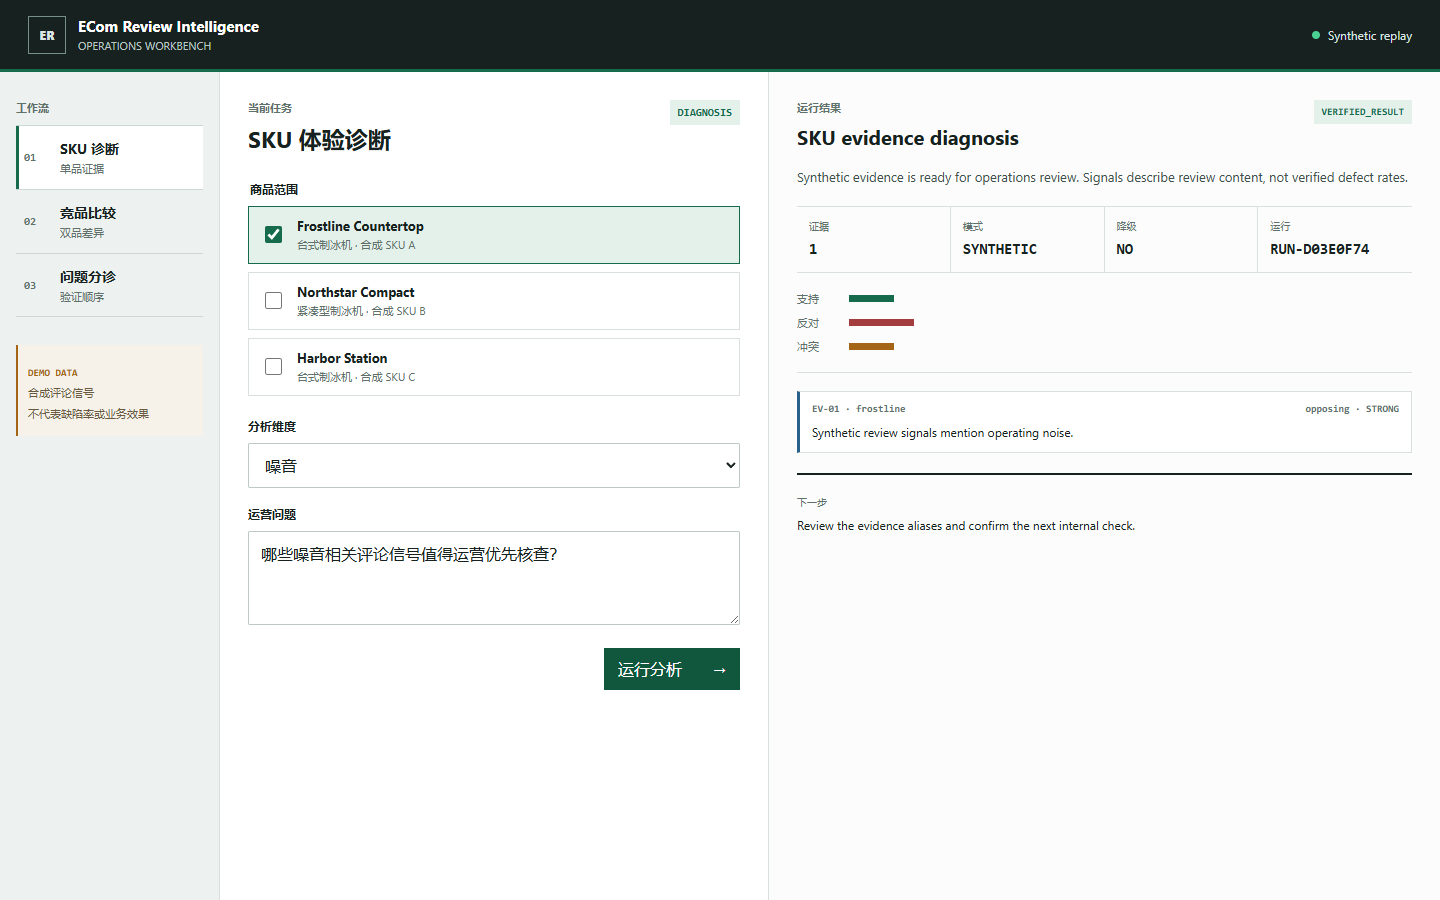
\includegraphics[width=\textwidth]{assets/p7-workbench-desktop.png}
  \caption{P7 synthetic 工作台电脑网页端。左侧选择任务，中间填写商品与问题，右侧查看状态、聚合信号、证据卡和下一步。截图只说明受控流程，不证明真人业务效果。}
  \label{fig:p7-desktop-integrated}
\end{figure}

左侧是任务导航，中间是表单，右侧是结果区。页面顶部会显示 synthetic 或 local，避免把演示数据误认为真实业务输出。

\subsection{3. 先学会看三个任务}

\textbf{SKU 体验诊断：}选择一个商品和一个维度，运行后先看状态，再看支持、反对和冲突信号，最后看优先核查项与匿名证据卡。

\textbf{竞品比较：}选择两个商品并使用同一维度，比较两边的聚合证据；结果不是购买推荐，也不是缺陷率。

\textbf{运营问题分流：}提交一个运营问题和允许比较的商品范围，结果帮助判断下一步由产品、客服或内容团队核实，不自动执行外部动作。

\subsection{4. 处理歧义并恢复}

标题命中多个候选时，状态变为 \texttt{NEEDS\_CLARIFICATION}。用户从已授权候选中选择后继续；服务用 P6 的 \texttt{checkpoint} 恢复原任务，不重新规划，也不能选择候选集合之外的商品。

\subsection{5. 读懂结果状态}

\begin{longtable}{>{\raggedright\arraybackslash}p{0.28\textwidth}>{\raggedright\arraybackslash}p{0.58\textwidth}}
\toprule
状态 & 先这样理解 \\
\midrule
\texttt{VERIFIED\_RESULT} & 当前结果通过本地规则、工具范围、Verifier 和引用门；是否行动仍由运营人员判断。 \\
\texttt{NEEDS\_CLARIFICATION} & 商品有歧义，需要在授权候选中选择，不代表程序故障。 \\
\texttt{DEGRADED\_SAFE\_RESULT} & 证据不足或检查未满足，系统给出受限结果，不补写结论。 \\
\texttt{FAILED} & 请求没有安全完成，应查看固定错误码和运行环境。 \\
\bottomrule
\end{longtable}

supporting、opposing、conflicting 是评论信号的聚合方向，不是缺陷率；evidence count 是本次允许使用的证据数量，不代表市场占比；优先核查项是下一步建议，不是自动决策。

\subsection{6. 何时使用 local 模式}

只有本地证据库、数据来路和 P6 回归均通过后，才运行：

\begin{lstlisting}
.\.venv\Scripts\python.exe scripts/run_phase7_local_regression.py --project-root .
.\.venv\Scripts\python.exe scripts/run_phase7_workbench.py --mode local --acknowledge-local-data --project-root . --port 8765
\end{lstlisting}

local 模式仍只允许浏览器看到聚合 DTO。公开截图和手册不能展示本地商品键、evidence id、路径或评论原文。

\section{问题、修复与验证}

问题包括 Host 和绝对路径扫描遗漏、旧 PASS 在失败后还存活、local 回归身份不足、工作台绕过 P6 Trace，以及自动化代替真人试用。修复包括闭集 Host/DTO、失败前失效旧工件、结构化 local 回执和真实浏览器入口验证；目标运营用户试用仍作为缺口保留，不能用开发者测试冒充。

\section{阶段产出与验收边界}

已完成的工程产出包括电脑网页端、typed API、synthetic 与受控 local adapter、电脑端截图、浏览器验证和公开聚合报告\filelink{docs/reports/phase-7-workbench-validation.md}。真人试用模板位于\filelink{docs/templates/p7-user-trial-record.md}。

P7 当前状态是 \texttt{IN\_PROGRESS}，即 \statusprogress。只有目标运营用户按模板完成任务、记录时间、证据复核和问题，才可以讨论易用性与业务价值。

\section{怎样进入下一阶段}

下一步是让真实目标用户分别完成手工流程和工作台流程，比较完成时间、错误、证据复核和主观负担，再决定权限、多人协作、监控和在线部署是否值得投入。

\section{面试怎么讲}

\begin{interviewbox}
“P7 不是给 CLI 套网页。我先定义浏览器公开 DTO，再把 synthetic 与显式 local adapter 分开，local 路径复用 P6 流程、工具和 Verifier。浏览器自动化和本地回归证明了工程接线，但目标运营用户结构化试用还没有完成，所以我不会声称已经节省工时或上线生产。”
\end{interviewbox}

\textbf{掌握标准：}能在电脑网页端完成三个任务，解释四种状态、公开 DTO 与内部 state 的边界，并准确说出 P7 为什么仍是 \texttt{IN\_PROGRESS}。
